
\thispagestyle{empty}

\newpage
{\Large \bf

  \noindent Supplementary Material\\

  \noindent 
 Effects of Tunable Hydrophobicity on the Collective Hydrodynamics of Janus Particles under Flows}\\

\noindent 
Szu-Pei Fu$^{1,*},$ 
Rolf Ryham$^{2},$ 
Bryan Quaife$^{3}$ and Y.-N. Young$^{4},$
\\

\noindent
$^{1}$Department of Mathematics, Trinity College, Hartford, Connecticut 06106, USA

\noindent
$^{2}$Department of Mathematics, Fordham University, Bronx, NY, USA

\noindent
$^{3}$Department of Scientific Computing, Florida State University, Tallahassee, Florida 32306, USA

\noindent
$^{4}$Department of Mathematical Sciences, New Jersey Institute of Technology, Newark, NJ 07102 USA
\\

\noindent $^*$Corresponding author. Address: Department of Mathematics, Trinity College, 
300 Summit Street, Hartford, CT 06106. email: \text{peter.fu@trincoll.edu}



\setcounter{page}{1}

\setcounter{figure}{0}
\renewcommand{\thefigure}{S\arabic{figure}}

\setcounter{equation}{0}
\renewcommand{\theequation}{S\arabic{equation}}

\setcounter{section}{0}
\renewcommand{\thesection}{S\arabic{section}} 


%-----ellipse repulsion--------------------

%\Phi_{\mathrm{rep}}

\section{Raw Data}




\begin{figure}[h!]
\begin{center}
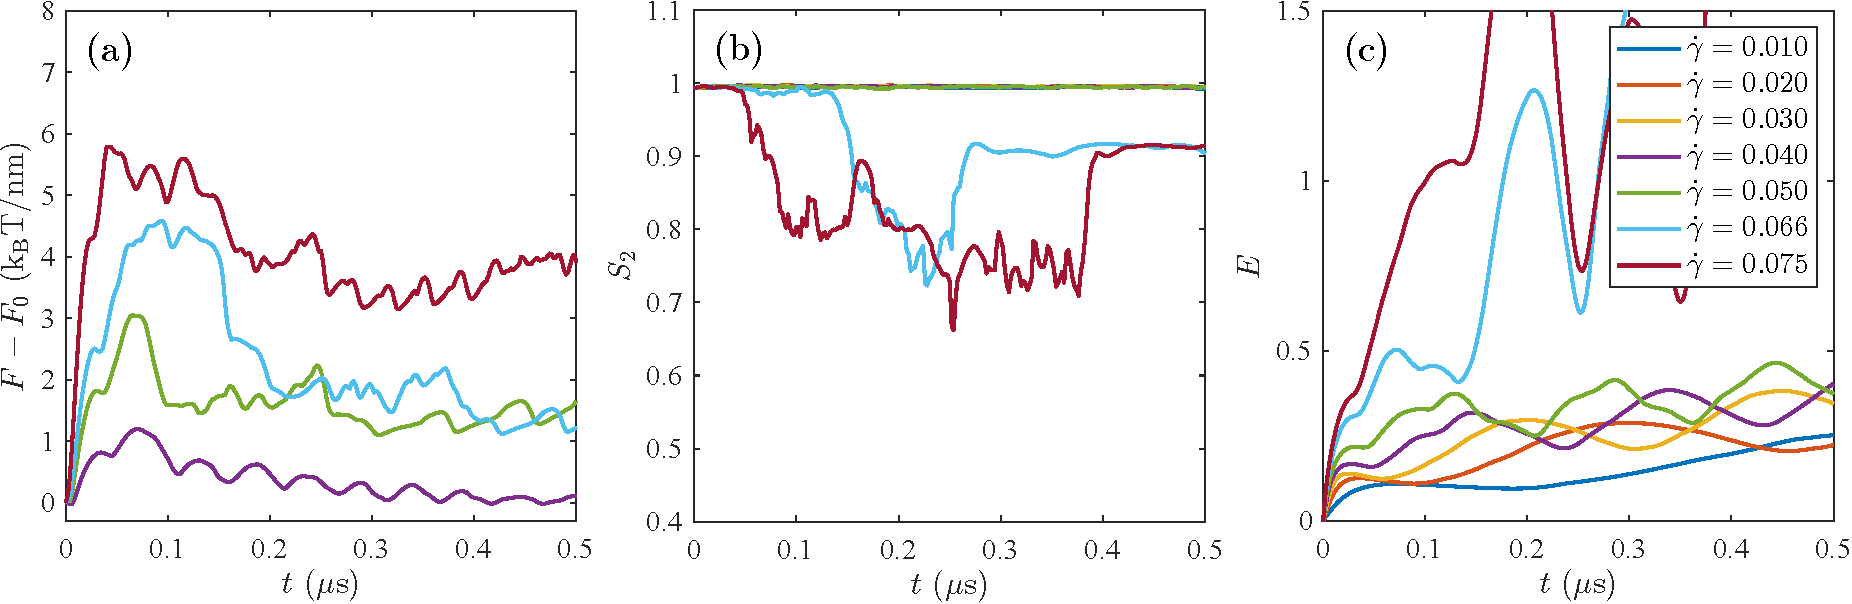
\includegraphics[width=\textwidth]{SMFigures/VeShRaw.pdf}
\end{center}
\caption{A Vesicle under a shear flow with choices of shear rates $\dot\gamma=0.01\sim0.075$. The change in free energy $F$ is plotted in panel (a). Panel (b) shows the scalar order parameter $S_2$ over time $t$. Panel (c) plots the change of strain parameter $E$ in percentage over time $t$. }
\label{fig:veshraw}
\end{figure}


\begin{figure}[h!]
\begin{center}
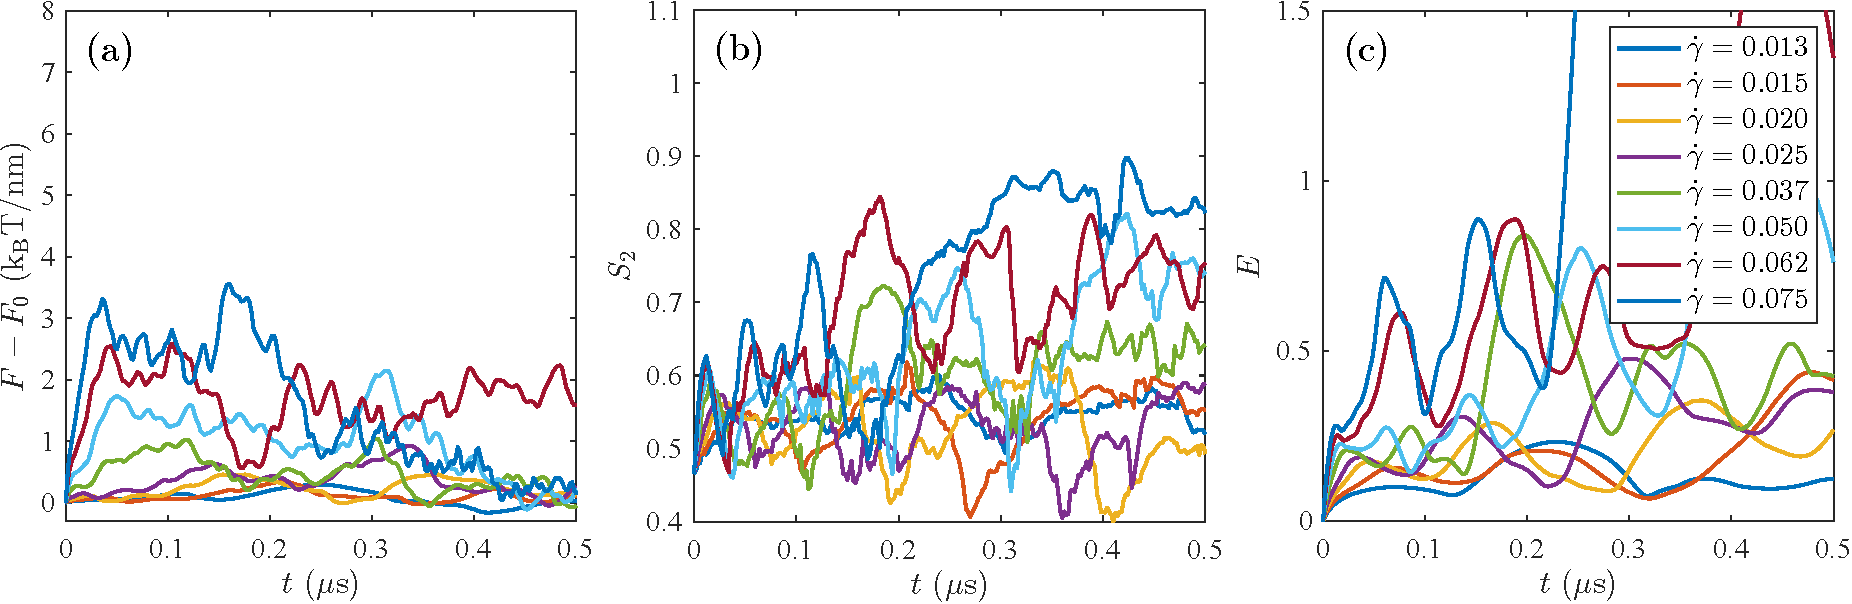
\includegraphics[width=\textwidth]{SMFigures/ULShRaw.pdf}
\end{center}
\caption{A unilamellar JP structure under a shear flow with choices of shear rates $\dot\gamma=0.013\sim0.075$. The change in free energy $F$ is plotted in panel (a). Panel (b) shows the scalar order parameter $S_2$ over time $t$. Panel (c) plots the change of strain parameter $E$ in percentage over time $t$. }
\label{fig:ulshraw}
\end{figure}



\begin{figure}[h!]
\begin{center}
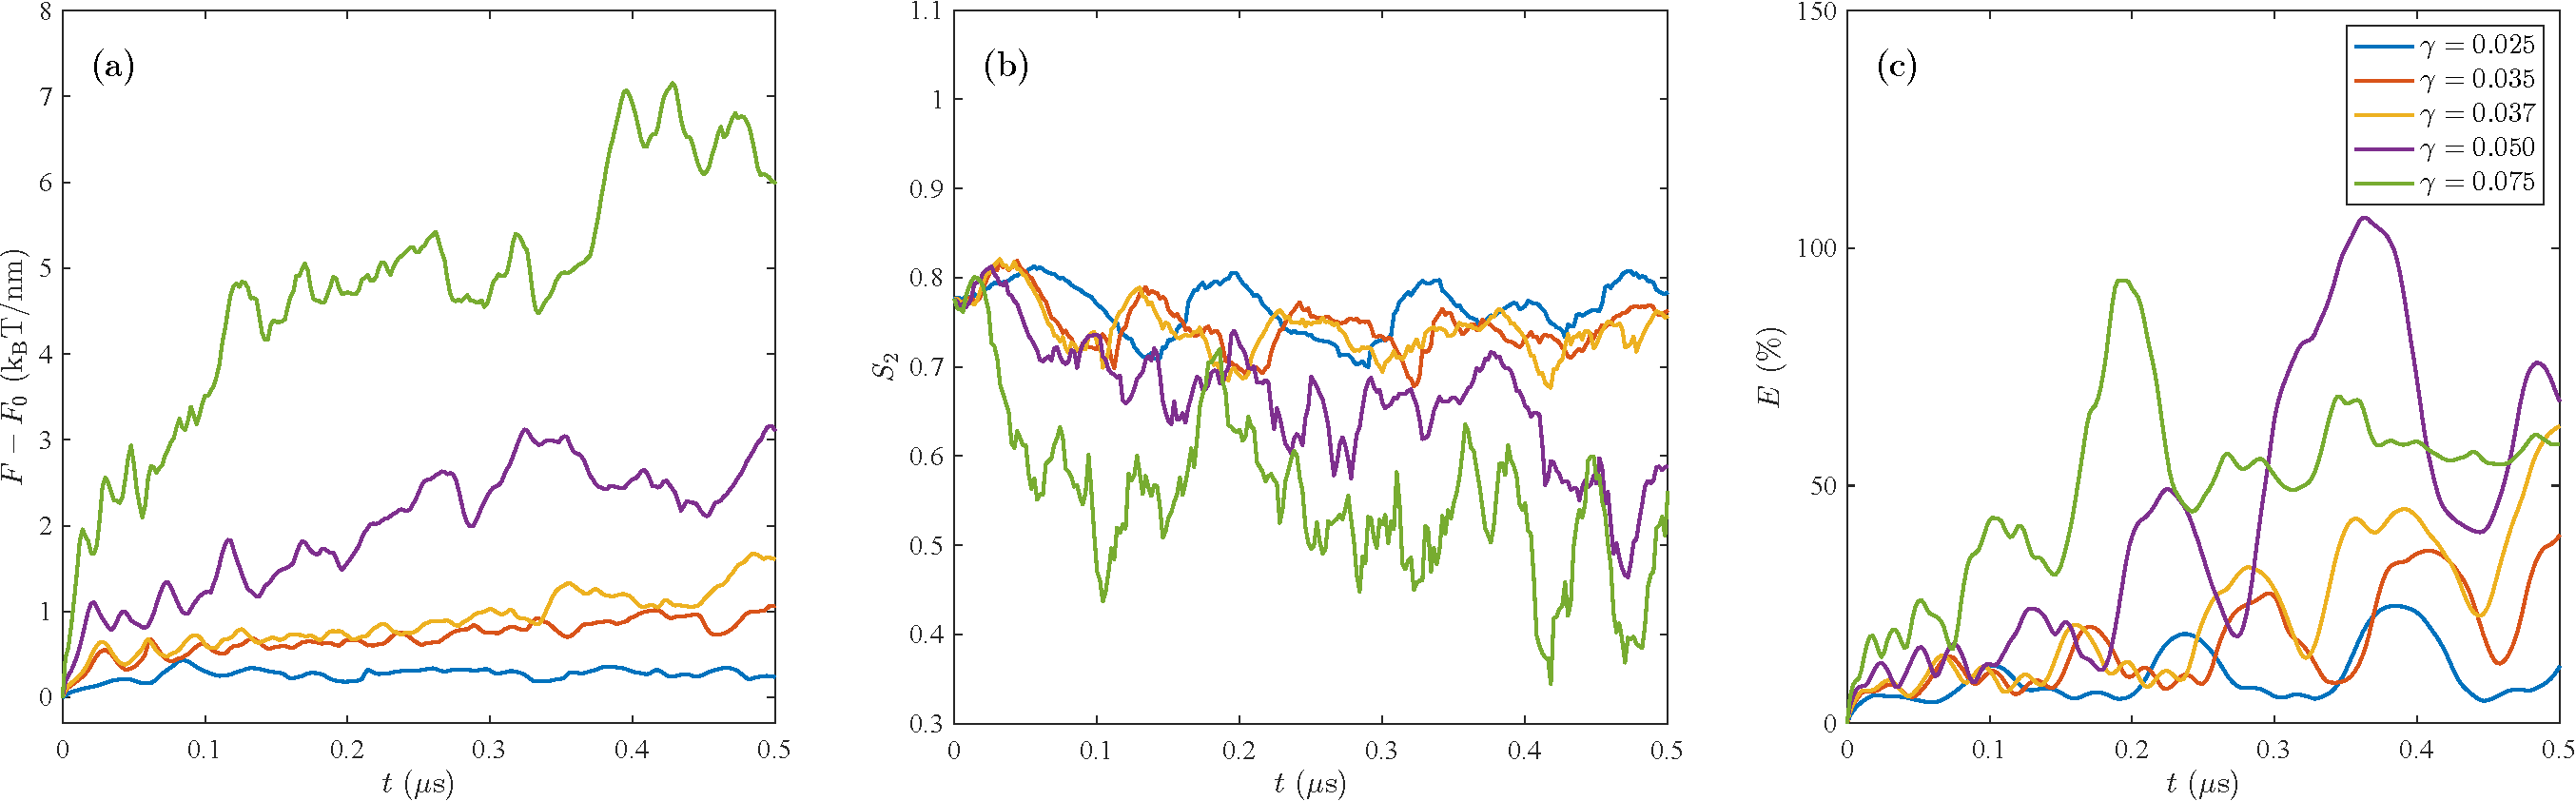
\includegraphics[width=\textwidth]{SMFigures/MLShRaw.pdf}
\end{center}
\caption{A multilamellar JP structure under a shear flow with choices of shear rates $\dot\gamma=0.025\sim0.075$. The change in free energy $F$ is plotted in panel (a). Panel (b) shows the scalar order parameter $S_2$ over time $t$. Panel (c) plots the change of strain parameter $E$ in percentage over time $t$. }
\label{fig:mlshraw}
\end{figure}


\begin{figure}[h!]
\begin{center}
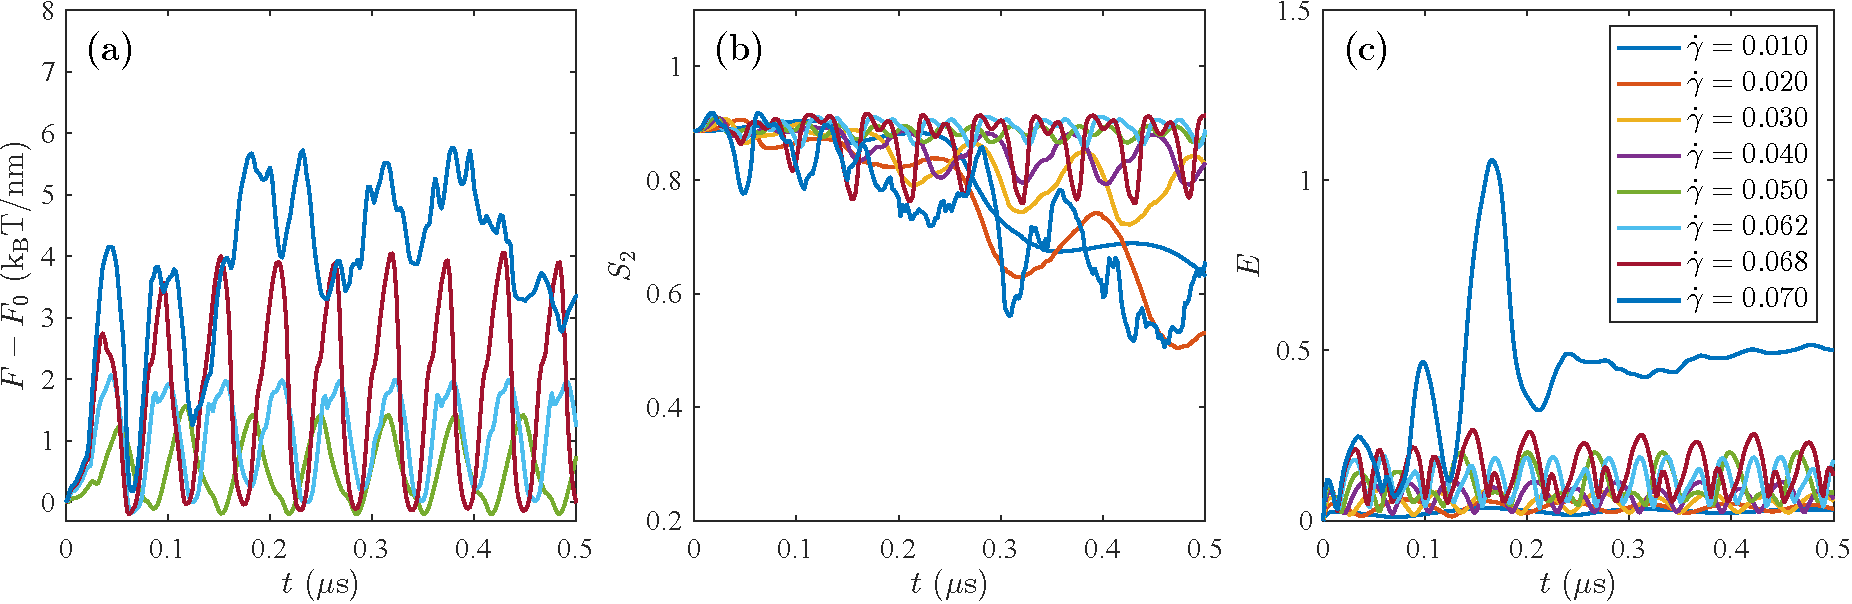
\includegraphics[width=\textwidth]{SMFigures/StShRaw.pdf}
\end{center}
\caption{A striated JP structure under a shear flow with choices of shear rates $\dot\gamma=0.01\sim0.07$. The change in free energy $F$ is plotted in panel (a). Panel (b) shows the scalar order parameter $S_2$ over time $t$. Panel (c) plots the change of strain parameter $E$ in percentage over time $t$. }
\label{fig:stshraw}
\end{figure}


\begin{figure}[h!]
\begin{center}
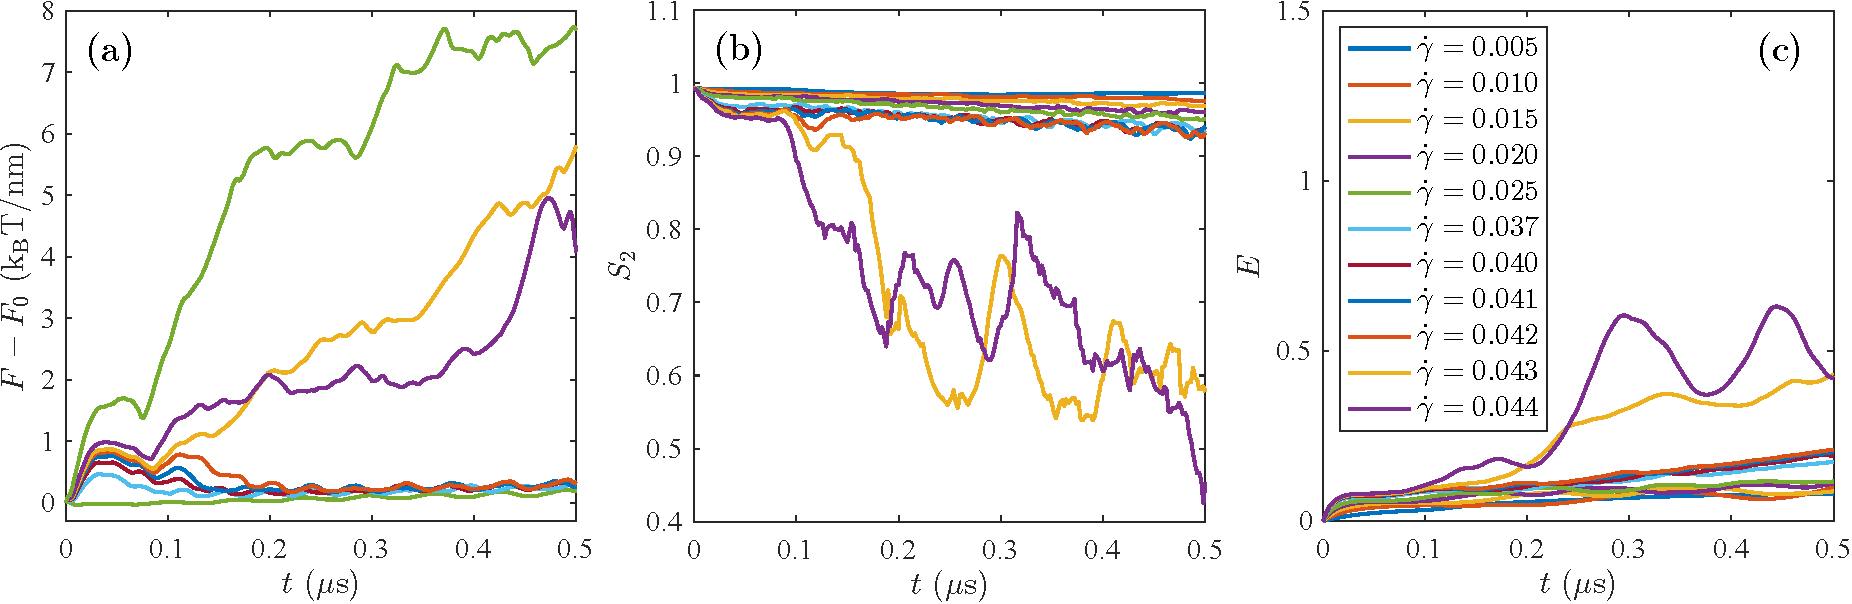
\includegraphics[width=\textwidth]{SMFigures/VeTGRaw.pdf}
\end{center}
\caption{A vesicle JP structure under a TG flow with choices of shear rates $\dot\gamma=0.005\sim0.044$. The change in free energy $F$ is plotted in panel (a). Panel (b) shows the scalar order parameter $S_2$ over time $t$. Panel (c) plots the change of strain parameter $E$ in percentage over time $t$. }
\label{fig:vetgraw}
\end{figure}



\begin{figure}[h!]
\begin{center}
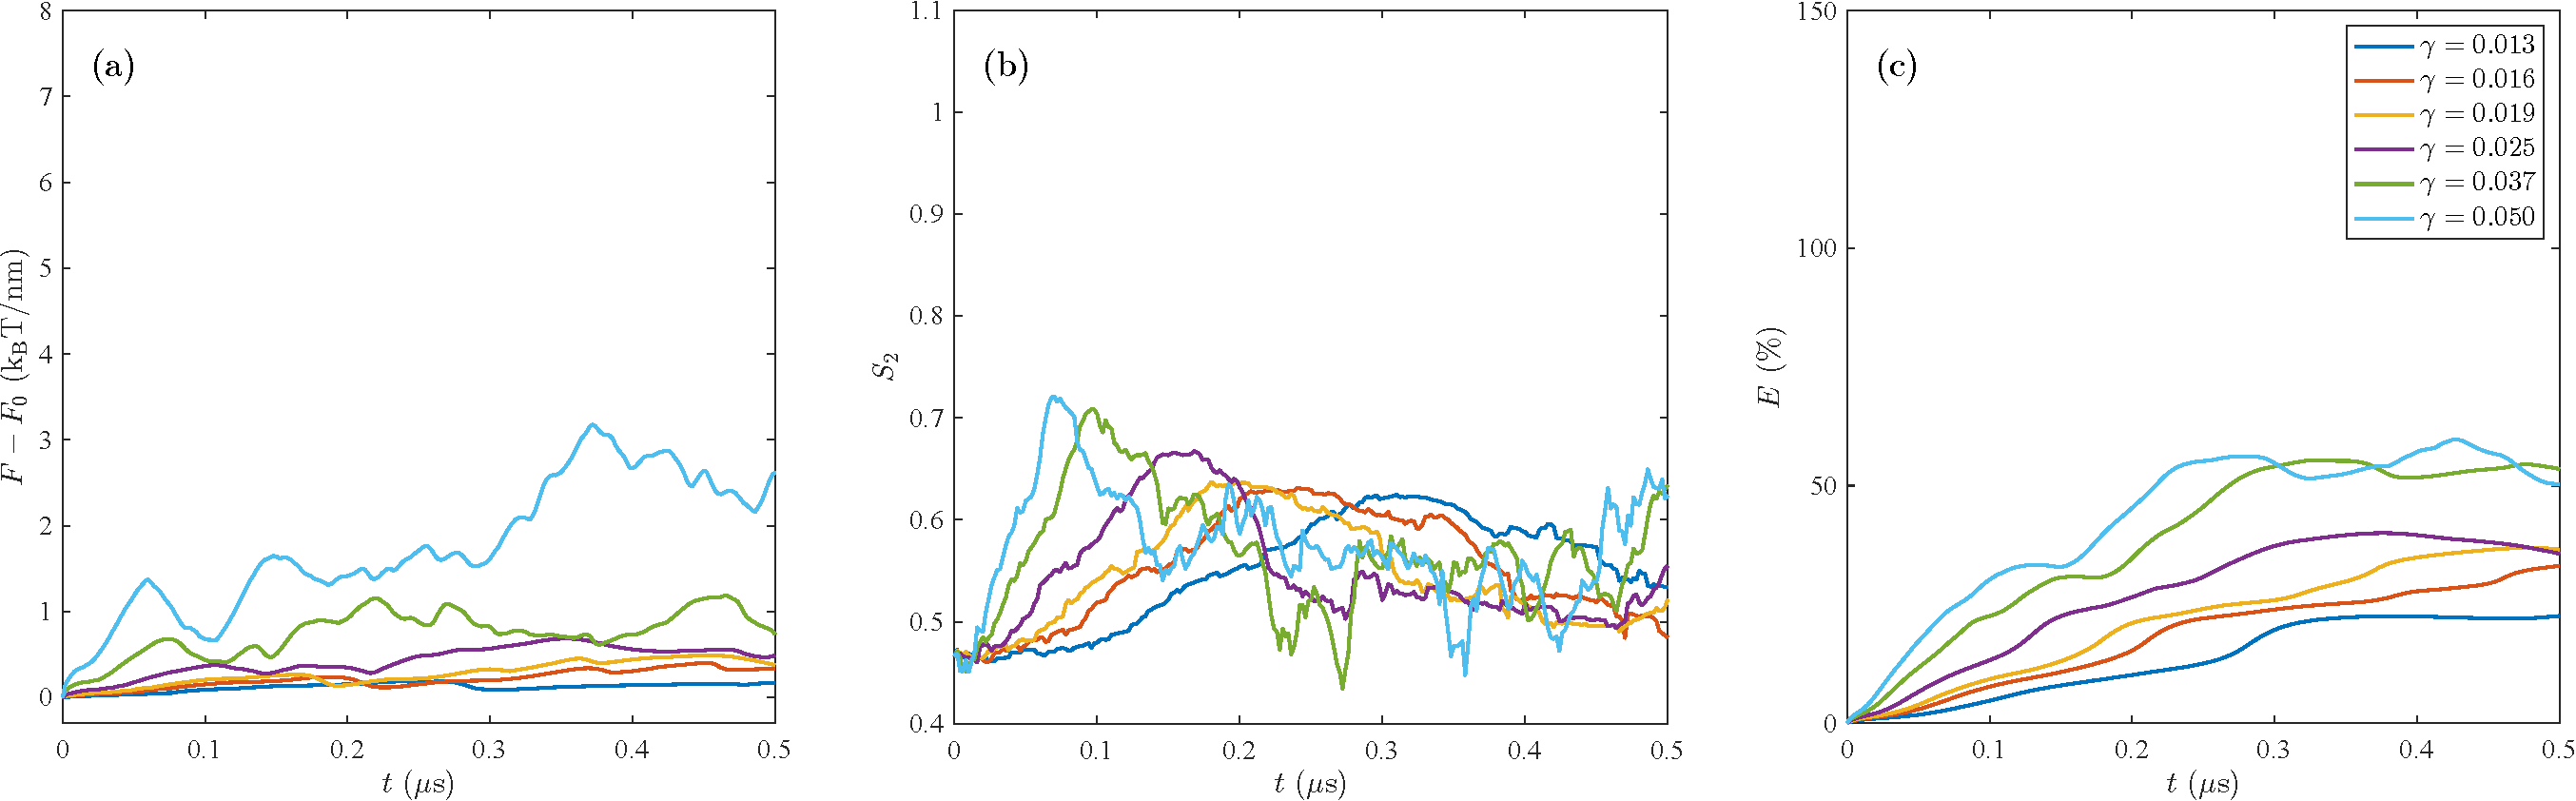
\includegraphics[width=\textwidth]{SMFigures/ULTGRaw.pdf}
\end{center}
\caption{A unilamellar JP structure under a TG flow with choices of shear rates $\dot\gamma=0.013\sim0.05$. The change in free energy $F$ is plotted in panel (a). Panel (b) shows the scalar order parameter $S_2$ over time $t$. Panel (c) plots the change of strain parameter $E$ in percentage over time $t$. }
\label{fig:ultgraw}
\end{figure}


\begin{figure}[h!]
\begin{center}
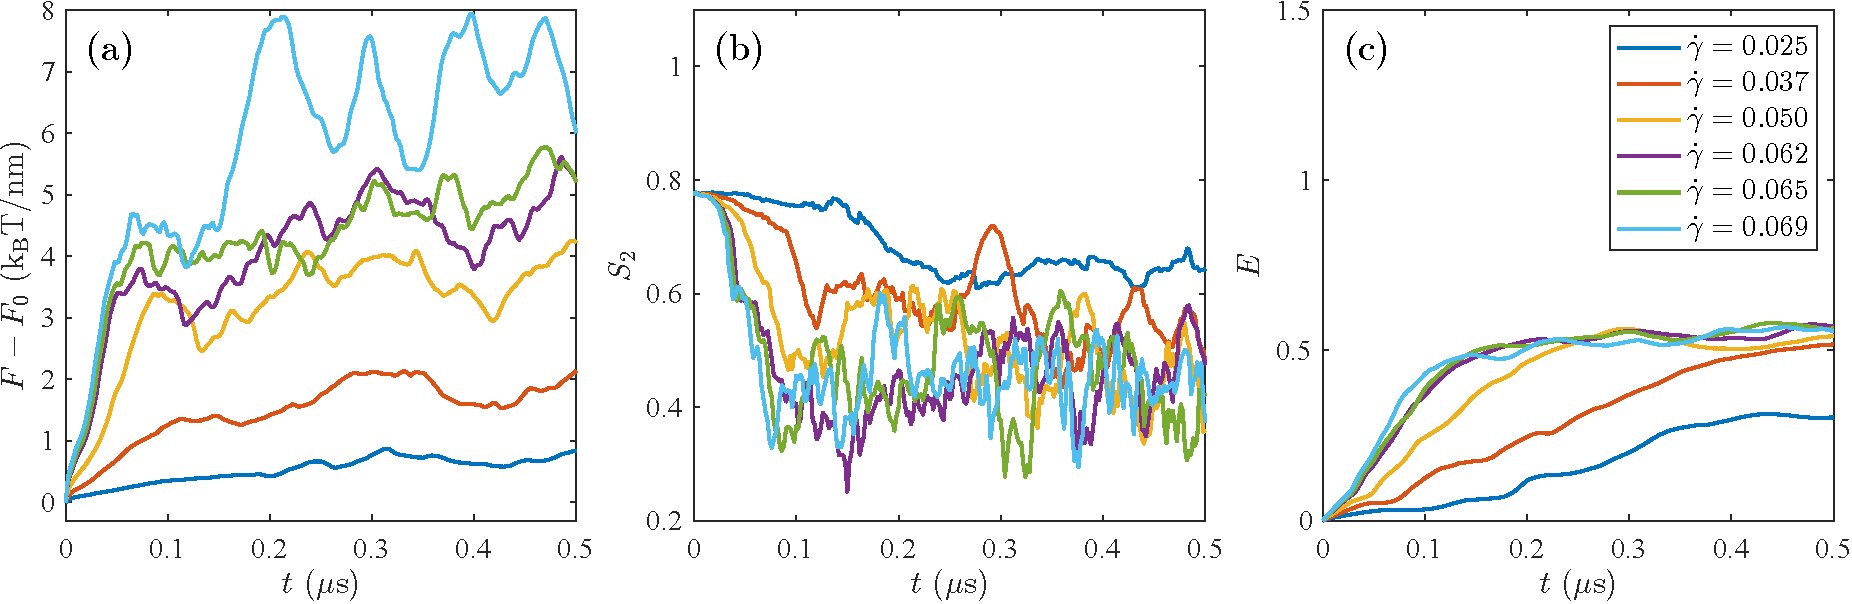
\includegraphics[width=\textwidth]{SMFigures/MLTGRaw.pdf}
\end{center}
\caption{A multilamellar JP structure under a TG flow with choices of shear rates $\dot\gamma=0.025\sim0.069$. The change in free energy $F$ is plotted in panel (a). Panel (b) shows the scalar order parameter $S_2$ over time $t$. Panel (c) plots the change of strain parameter $E$ in percentage over time $t$. }
\label{fig:mltgraw}
\end{figure}


\begin{figure}[h!]
\begin{center}
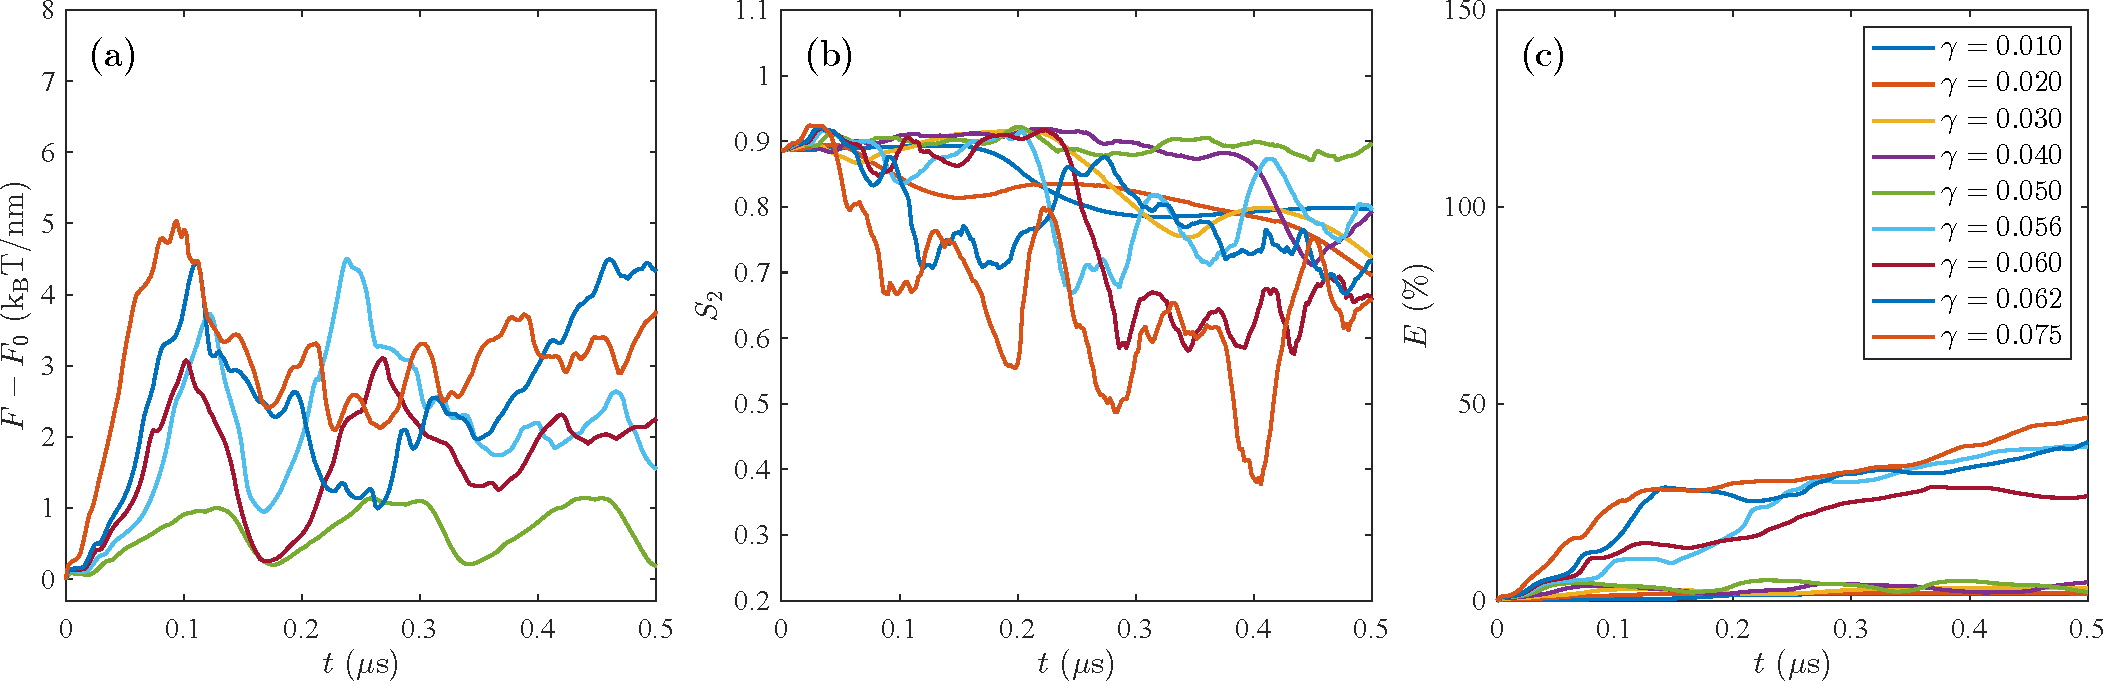
\includegraphics[width=\textwidth]{SMFigures/StTGRaw.pdf}
\end{center}
\caption{A striated JP structure under a TG flow with choices of shear rates $\dot\gamma=0.01\sim0.069$. The change in free energy $F$ is plotted in panel (a). Panel (b) shows the scalar order parameter $S_2$ over time $t$. Panel (c) plots the change of strain parameter $E$ in percentage over time $t$. }
\label{fig:mltgraw}
\label{fig:sttgraw}
\end{figure}

\sloppy
\section{Movie Captions}\mbox{} \\

\noindent
{\bf Movie S1. Relaxation} 
There are 60 circular particles with radius 1.25~nm that are initially
confined in a square box. The simulation results show the relaxation
with each of the three boundary conditions. The time step of all
simulations is $\Delta t=0.2$. The color on the boundary from blue to
red is for $\min g(\xx)$ to $\max g(\xx)$. All final configurations are
adopted in simulations with hydrodynamic flows. \\


\noindent
{\bf Movie S2. Structures in a Shear Flow without Ruptures} 
We adopt the relaxed configurations and place the JP structures in the
shear flow. For the choices of the shear rate, we pick: $\dot\gamma =
0.05$ for the vesicle, $\dot\gamma = 0.05$ for the bilayer, $\dot\gamma
= 0.05$ for the multi-lamellar, and $\dot\gamma = 0.1$ for the striated
configurations. The vesicle case undergoes tank-treading whereas the
initially disordered BC (i) case increases orientational order. The
multilamellar assemply behaves as a rigid body, and the striated
configuration moreso. No ruptures occur. \\



\noindent
{\bf Movie S3. Structures in a Taylor-Green Flow without Ruptures} 
We adopt the relaxed configurations and place the JP structures in the
Taylor-Green flow at low flow rates. For the choices of the flow
strength, we pick: $V_0 = 0.1$ for the vesicle, $V_0 = 0.1$ for the
disordered bilayer, $V_0 = 0.1$ for the multi-lamellar, and $V_0 = 0.2$
for the striated configurations. The vesicle stays inact, whereas the
dissordered bilayer is pulled apart. Like in Supplementary Movie S2, the
striated assembly is basically rigid. \\


\noindent
{\bf Movie S4. Structures in a Shear Flow with Ruptures} 
We adopt the relaxed configurations and place the JP structures in the
shear flow at a higher shear rate. For the choices of the shear rate, we
pick: $\dot\gamma = 0.075$ for the vesicle, $\dot\gamma = 0.1$ for the
bilayer, $\dot\gamma = 0.15$ for the multi-lamellar, and $\dot\gamma =
0.15$ for the striated configurations. The time step of all simulations
is $\Delta t=0.2$. In this movie, some clear structural ruptures occur
in each case. In order to observe the structure behaviors at later time,
we stabilize the frame by tracking the center of mass position of all
JP. \\


\noindent
{\bf Movie S5. Structures in a Taylor-Green Flow with Ruptures} 
We adopt the relaxed configurations and place the JP structures in the
Taylor-Green flow at higher flow rates. For the choices of the flow
strength, we pick: $V_0 = 0.2$ for the vesicle, $V_0 = 0.2$ for the
bilayer, $V_0 = 0.2$ for the multi-lamellar, and $V_0 = 0.3$ for the
striated configurations. Clear structural ruptures occur in each case.
In all cases, there is significant reduction in the orientational order
of the assemblies. While the BC (i) cases are broken into several
pieces, the main body of the BC (ii) and BC (iii) assemblies are not
pulled apart by the background flow. 

